%%% This file is part of the Open HörTech Master Hearing Aid (openMHA)
%%% Copyright © 2019 HörTech gGmbH
%%%
%%% openMHA is free software: you can redistribute it and/or modify
%%% it under the terms of the GNU Affero General Public License as published by
%%% the Free Software Foundation, version 3 of the License.
%%%
%%% openMHA is distributed in the hope that it will be useful,
%%% but WITHOUT ANY WARRANTY; without even the implied warranty of
%%% MERCHANTABILITY or FITNESS FOR A PARTICULAR PURPOSE.  See the
%%% GNU Affero General Public License, version 3 for more details.
%%%
%%% You should have received a copy of the GNU Affero General Public License, 
%%% version 3 along with openMHA.  If not, see <http://www.gnu.org/licenses/>.

% Latex header for doxygen 1.8.11
% adapted for openMHA
\documentclass[11pt,a4paper,twoside]{article}

% Packages required by doxygen
\usepackage{fixltx2e}
\usepackage{calc}
\usepackage{../openMHAdoxygen}
\setlength{\headheight}{13.6pt}
\usepackage[export]{adjustbox} % also loads graphicx
\usepackage{graphicx}
\usepackage[utf8]{inputenc}
\usepackage{makeidx}
\usepackage{multicol}
\usepackage{multirow}
\PassOptionsToPackage{warn}{textcomp}
\usepackage{textcomp}
\usepackage[nointegrals]{wasysym}
\usepackage[table]{xcolor}

% Font selection
\usepackage[T1]{fontenc}
\usepackage{helvet}
\usepackage{courier}
\usepackage{amssymb}
\usepackage{sectsty}
\renewcommand{\familydefault}{\sfdefault}
\allsectionsfont{%
  \fontseries{bc}\selectfont%
  \color{darkgray}%
}
\renewcommand{\DoxyLabelFont}{%
  \fontseries{bc}\selectfont%
  \color{darkgray}%
}
\newcommand{\+}{\discretionary{\mbox{\scriptsize$\hookleftarrow$}}{}{}}

% Headers & footers
\usepackage{fancyhdr}
\pagestyle{fancyplain}
\renewcommand{\sectionmark}[1]{%
  \markright{\thesection\ #1}%
}
\fancyhead[LE]{\fancyplain{}{\bfseries\thepage}}
\fancyhead[CE]{\fancyplain{}{}}
\fancyhead[RE]{\fancyplain{}{\bfseries\leftmark}}
\fancyhead[LO]{\fancyplain{}{\bfseries\rightmark}}
\fancyhead[CO]{\fancyplain{}{}}
\fancyhead[RO]{\fancyplain{}{\bfseries\thepage}}
\fancyfoot[LE]{\fancyplain{}{}}
\fancyfoot[CE]{\fancyplain{}{}}
\fancyfoot[RE]{\fancyplain{}{\bfseries\scriptsize \copyright{} 2019 H\"orTech gGmbH, Oldenburg }}
\fancyfoot[LO]{\fancyplain{}{\bfseries\scriptsize \copyright{} 2019 H\"orTech gGmbH, Oldenburg }}
\fancyfoot[CO]{\fancyplain{}{}}
\fancyfoot[RO]{\fancyplain{}{}}

% Indices & bibliography
\usepackage{natbib}
\usepackage{tocloft}
\setcounter{tocdepth}{2}
\setcounter{secnumdepth}{4}
\addtolength{\cftsubsecnumwidth}{5pt}
\makeindex

% Custom commands
\newcommand{\clearemptydoublepage}{%
  \newpage{\pagestyle{empty}\cleardoublepage}%
}

\usepackage{caption}
\captionsetup{labelsep=space,justification=centering,font={bf},singlelinecheck=off,skip=4pt,position=top}

\setlength\parindent{0pt}
\usepackage{hyperref}
\usepackage[hang,flushmargin]{footmisc}
\usepackage[margin=1in]{geometry}
\usepackage{color}
\usepackage{subcaption}

\begin{document}
\MHAtitle{Getting Started}
\newpage
\MHAcopyright{}
\newpage
\tableofcontents
\newpage
\pagenumbering{arabic}


\begin{comment}
windows --interactive mode?

\end{comment}




\begin{comment}
\section{Introduction - What is openMHA?}

The large incidence rate of hearing loss (about 13\% of the US population), its high economic costs and the limitations of technical rehabilitative solutions call for an effort towards improving the rehabilitation of hearing impairment. The major aim of the envisaged project is therefore to facilitate research and development towards new technical solutions that improve rehabilitative devices. To achieve this, a large group of researchers will be provided with the means to efficiently develop and evaluate, in collaborative multi-center environments, novel signal processing schemes, individualized fitting procedures, technical solutions and services for hearing devices such as hearing aids and assistive listening devices. This approach leads to more integrated, sustainable and focused research towards improving hearing devices in general. [kopiert von Website, weglassen?, anpassen?] \\
\end{comment}

\begin{comment}
\textcolor{orange}{\textbf{Note: There are some sections which differ from each other depending on your operating system and some which do not. The system-dependent sections will be indicated with the * - symbol. }}
\end{comment}





\section{Requirements}
\subsection{Required Programs}
\label{subsec:required_prog}

\textcolor{orange}{\textbf{Before using the starting guide the following software should already be installed:}}

\begin{itemize}
   \item \large{{openMHA}}   \\
     \footnotesize{\url{https://github.com/HoerTech-gGmbH/openMHA/releases}} 
   %\item \large{{jack\_playrec}} \\
   %\footnotesize{\url{https://github.com/HoerTech-gGmbH/jack\_playrec/blob/master/INSTALLATION.md}}
   \item \large{{Matlab or Octave}}    \\
     \footnotesize{\url{https://de.mathworks.com/downloads/}} \\
     \footnotesize{\url{https://www.gnu.org/software/octave/download.html}}
   \item \large{{JACK Audio Connection Kit}}
   \begin{itemize}
   \item \textcolor{orange}{\textbf{Linux:}} \\
   $\rightarrow$ {\ttfamily sudo apt-get install jackd2} \\
   $\rightarrow$ {\ttfamily sudo apt-get install qjackctl}
   \item \textcolor{orange}{\textbf{Windows}} \\
   \footnotesize{\url{http://jackaudio.org/downloads/}}
   \item \textcolor{orange}{\textbf{MacOS}} \\
   \footnotesize{\url{http://jackaudio.org/downloads/}} %\\ or \\
   %\footnotesize{\url{http://www.jackosx.com/download.html}}
   \end{itemize}
\end{itemize}

\subsection{Path Setup (\textcolor{orange}{Windows only})}
\label{subsec:windows_path_setup}

\begin{itemize}
\item \textbf{Rightclick Windows "Start" Icon} $\rightarrow$ \textbf{System} $\rightarrow$ search for \textbf{Erweiterte Systemeinstellungen anzeigen} $\rightarrow$ \textbf{Umgebungsvariablen} $\rightarrow$ \textbf{Systemvariablen} $\rightarrow$ look for variable \textbf{"Path"} $\rightarrow$ \textbf{Bearbeiten} $\rightarrow$ \textbf{Neu} $\rightarrow$ type in \textbf{C:\textbackslash Program Files\textbackslash openMHA\textbackslash bin\textbackslash} $\rightarrow$ close all open windows by pressing \textbf{OK}
\end{itemize}

\newpage

\subsection{Update to Latest Version}


Make sure that you are using the latest version of openMHA. You can install the new version by:

\begin{itemize}
   \item \textcolor{orange}{\textbf{Linux:}} \\
   $\rightarrow$ {\ttfamily sudo apt-get install \texttt{-{}-}only-upgrade openmha} 
   \item \textcolor{orange}{\textbf{Windows}} \\
   \footnotesize{\url{https://github.com/HoerTech-gGmbH/openMHA/releases}}
   \item \textcolor{orange}{\textbf{MacOS}} \\
   \footnotesize{\url{https://github.com/HoerTech-gGmbH/openMHA/releases}}
   \end{itemize}



 


%\item A folder containing openMHA application examples was generated during the openMHA installation progress. This folder can be found in \textbf{C:\textbackslash Program Files\textbackslash openMHA\textbackslash examples}. In order to edit and work with these examples it is required to copy and paste them to a folder which is not protected, e.g. \textbf{C:\textbackslash Users\textbackslash YourUserName\textbackslash Documents}.


\section{Getting Started}

    \subsection{Starting openMHA}
    \label{starting_openmha}
    
After installing openMHA (download link: see section \ref{subsec:required_prog}) you can start openMHA by: 

\subsubsection*{\textcolor{orange}{\textbf{Linux}}}

In order to start openMHA open your \textbf{terminal} and type: \\
$\rightarrow$ {{\ttfamily \textbf{mha \texttt{-{}-}interactive}} 


\subsubsection*{\textcolor{orange}{Windows}}}
Make sure that you did the path setup from section \ref{subsec:windows_path_setup}.
In windows you can open your \textbf{terminal} by: \\ \\
$\rightarrow$ "\textbf{Windows + R}" \\
    $\rightarrow$ type in {{\ttfamily \textbf{cmd}}} and press \textbf{Enter} \\
    Type now {{\ttfamily \textbf{mha \texttt{-{}-}interactive}}  into the terminal window. 
   


\subsubsection*{\textcolor{orange}{MacOS}}

Open your \textbf{terminal} by pressing \textbf{Command + Space} in order to open spotlight search, type "terminal" and press enter. Type: \\ \\
$\rightarrow$ {{\ttfamily \textbf{mha \texttt{-{}-}interactive}} \\ \\ in your \textbf{terminal}.\\


\begin{figure}[H]
\centering
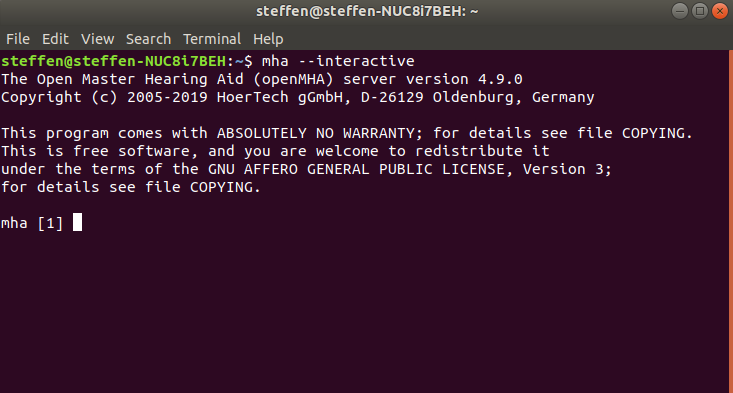
\includegraphics[scale=0.4]{mha_interactive.png}
\caption{- Linux Terminal: Type {{\ttfamily \textbf{mha \texttt{-{}-}interactive}}}}
\end{figure}


\dotfill \\

\large{\textbf{Note}}: It does matter in which directory openMHA is started! This is very important to understand for later tasks: If you are using your console \\ e.g. in \textit{/home/YourUserName/Documents/workshop/}, by typing {{\ttfamily \textit{mha \texttt{-{}-}interactive}}, openMHA will be started in \textbf{this} directory! You can start openMHA from any path you want. \\


\textcolor{orange}{\textbf{You have managed to start openMHA. In the next section there will be a step-by-step tutorial on how to use a simple configuration.}}

\vspace{1cm}





\newpage
\begin{comment}
\section{Use Matlab Function "jack\_playrec" to Communicate with JACK Server}   

One possibility to transfer audio signals to a JACK server is the jack\_playrec. To do this following the steps below:

\begin{enumerate}
\item Start a JACK server (sample rate = 44100)
\item Check if you already followed the instructions from \textbf{section \ref{sec:beforeplayrec}}
    \item \textbf{Start Matlab} 
    \item \textbf{Go to} $\rightarrow$ \textbf{/Users/usr/local/lib YourUserName/usr/local/lib Documents/usr/local/lib jack-playrec/usr/local/lib mfiles} using the Matlab \textbf{"Current Folder"} Section
    
    You can now copy the following lines of code into the Matlab command windows. This simple code below shows a minimal example of how to send an audio signal to a JACK client (here system:playback\_1). 


\begin{verbatim}
sampling_rate = 44100; %needs to fit sample rate of JACK server
frequency = 440; %Frequency in Hertz
signal_duration = 1; %Signal duration in seconds

t= 0:1./sampling_rate:signal_duration-1./sampling_rate;
sinus = transpose(sin(2*pi*frequency*t));
jack_playrec(sinus,'output',{'system:playback_1'});
\end{verbatim}  

\end{enumerate}


\newpage
\end{comment}

\section{Step-by-Step Exercise: Gain Application}

\textbf{First Steps}
\label{sec:first_steps}

A simple openMHA configuration is the gain application. The corresponding parameters (e.g. gain factor, input channels, fragment size and sample size) can be set manually, however for this examples there is already a configuration script available under: 
\begin{itemize}
\item \textcolor{orange}{\textbf{Linux}}: \textit{/usr/share/openmha/examples/00-gain} 
\item \textcolor{orange}{\textbf{Windows}}: \textit{C:\textbackslash Program Files\textbackslash openMHA\textbackslash examples\textbackslash 00-gain}
\item \textcolor{orange}{\textbf{MacOS}}: \textit{/usr/local/share/openmha/examples/00-gain} 
\end{itemize}

If you are curious what each line of the configuration script means you can read the comments which are denoted by \#. For now we will just use the configuration script, which was already created for demontration purposes. In order to use the configuration file, do the following steps:

\dotfill \\

\begin{enumerate}
    \item \textbf{Close all} running openMHA processes
    
    \item \textbf{Copy} the examples folder from the protected directory
    \\ (e.g. /usr/share/openmha/examples/) (\textcolor{orange}{\textbf{see above for your specific operating system}})
   
\begin{figure}[H]
\centering
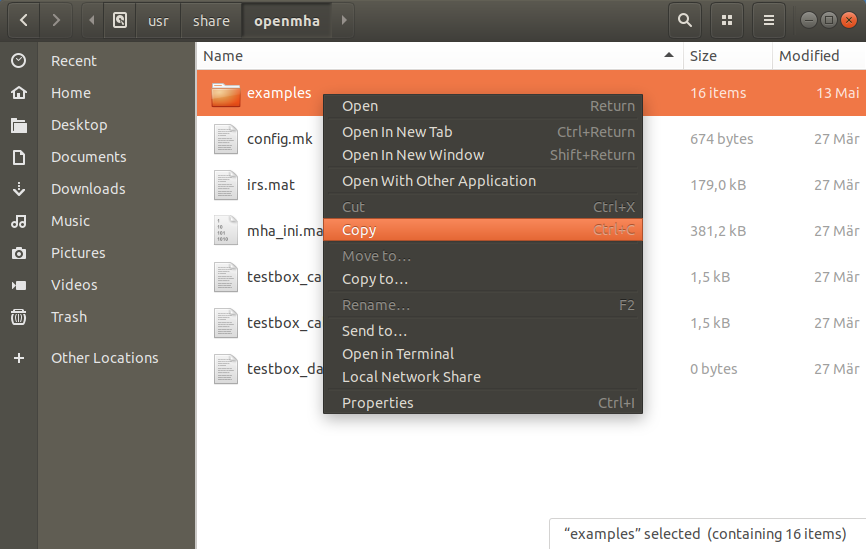
\includegraphics[scale=0.3]{copy_examples.png}
\caption{- Copy the examples folder from the protected directory (e.g. /usr/share/openmha/}
\end{figure}

\item \textbf{Paste} the examples into folder within a non-protected directory, e.g.:

	\begin{itemize}
\item \textcolor{orange}{\textbf{Linux}}: \textit{/home/YourUserName/Documents/} 
\item \textcolor{orange}{\textbf{Windows}}: \textit{\textbackslash Users\textbackslash YourUserName\textbackslash Documents\textbackslash } 
\item \textcolor{orange}{\textbf{MacOS}}: \textit{/Users/YourUserName/Documents/} 
\end{itemize} 

\begin{figure}[H]
\centering
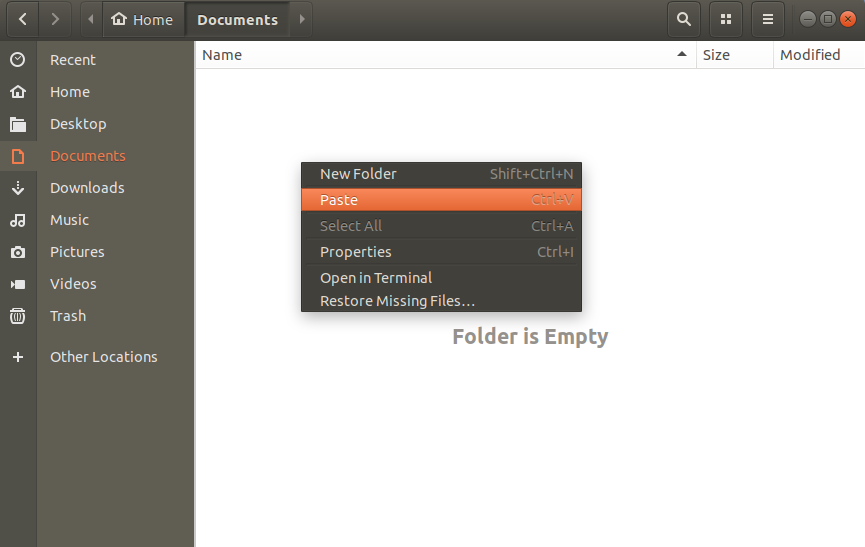
\includegraphics[scale=0.3]{paste_examples.png}
\caption{- Paste examples into folder inside a non-protected directory (e.g. /home/YourUserName/Documents}
\end{figure}
    
    
    \item Open your \textbf{terminal} (see \ref{starting_openmha})
    \item \textbf{Navigate inside the examples folder into the subdirectory of the first example $\rightarrow$ \textbf{00-gain}} \\ (e.g. \textit{/home/YourUserName/Documents/examples/00-gain} )\\ \\
    $\rightarrow$ you can use \textbf{cd ..} to navigate one folder level higher \\
    $\rightarrow$ and \textbf{cd foldername} to navigate one folder level down
    \item Type {{\ttfamily mha \texttt{-{}-}interactive}} and press \textbf{Enter}
\end{enumerate}

\subsection{Static Audio File}

Since you are now connected to openMHA you can type in commands. In order to read in the configuration file \textbf{gain.cfg} (which lies directly in \textit{00-gain}), type: \\

%$\rightarrow${\ttfamily ?read:\textbackslash Users\textbackslash YourUserName\textbackslash Documents\textbackslash examples\textbackslash 00-gain\textbackslash gain.cfg}
$\rightarrow${\ttfamily ?read:gain.cfg}


%with the corresponding file directory of gain.cfg. 
Run the script by:

$\rightarrow$ {\ttfamily cmd=start}

and close it by typing:

$\rightarrow$ {\ttfamily cmd=quit} 
\\

\begin{figure}[H]
\centering
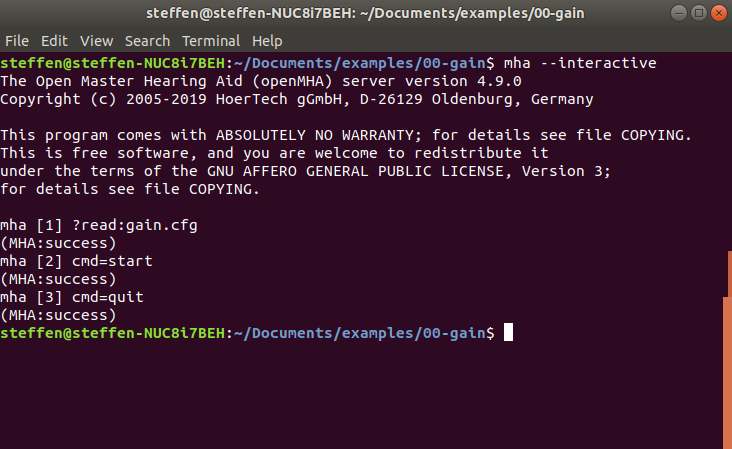
\includegraphics[scale=0.4]{static_gain.png}
\caption{Interactive mode: Applying gain to a static audio signal}
\end{figure}

\textcolor{orange}{\textbf{After quitting the openMHA process a second .wav file "1speaker\_diffNoise\_2ch \\ \_OUT.wav" should have appeared within the folder you are working in. (e.g. \textit{/home/YourUserName/Documents/examples/00-gain}). You can listen to it and compare it to "1speaker\_diffNoise\_2ch.wav".}}

\newpage

\subsection{Starting openMHA with JACK Input/Output}

In this section the configuration settings described in the previous section will be used while using a JACK server as audio backend. This means that we can apply a gain to e.g. our microphone input in real time. In order to set up and connect a JACK server you can follow the steps below:

\begin{enumerate}
    \item \textbf{Start Jack Audio Connection Kit} 
    
    \begin{itemize}
\item \textcolor{orange}{\textbf{Linux}}: \\ Type {\ttfamily qjackctl} into your \textbf{terminal} 
\item \textcolor{orange}{\textbf{Windows}}: \\ Use the \textbf{JACK Control} Icon
\item \textcolor{orange}{\textbf{MacOS}}: \\ \textbf{Start} the \textbf{Jack Audio Connection Kit} GUI by starting the \textit{qjackctl} application found in \textit{/Applications/Jack/}.
\end{itemize}

\begin{figure}[H]
\centering
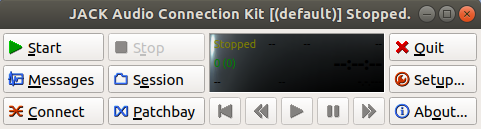
\includegraphics[scale=0.4]{jack_gui.png}
\caption{JACK Audio Connection Kit: GUI}
\end{figure}
      
    \item \textbf{Setup} $\rightarrow$ \textbf{Settings} $\rightarrow$ select proper Driver, Interface, Sample Rate=44100, \\Frames/Period=64 $\rightarrow$ \textbf{OK} 
    
\begin{figure}[H]
\centering
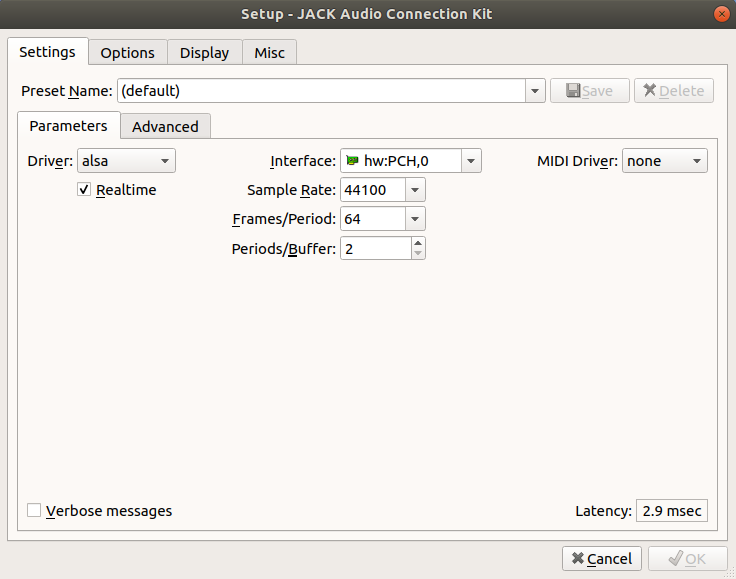
\includegraphics[scale=0.4]{jack_setup.png}
\caption{Jack GUI: Setup}
\end{figure}
    \item Click \textbf{Start} for starting a JACK server $\rightarrow$ Check \textit{Messages} for any errors (sometimes it can be difficult to find proper driver settings, try out different settings) \\
    
\begin{figure}[H]
\centering
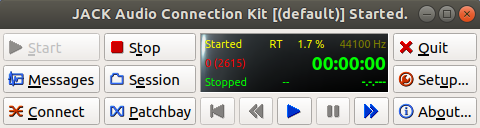
\includegraphics[scale=0.4]{jack_started.png}
\caption{Jack GUI with running server}
\end{figure}

    %\textcolor{red}{\textbf{For MacOs Users: If you encounter any problem using JACK you can try \textit{\textbf{JackPilot}}, you can find the download link in section \ref{subsec:required_prog}}}
    


\item In order to test your Jack server, you can go to the \textbf{Connect} section and connect the inputs of your (internal) microphones to the output channels of the jack server. (See Figure \ref{fig: jack_connection})

\begin{figure}[H]
\centering
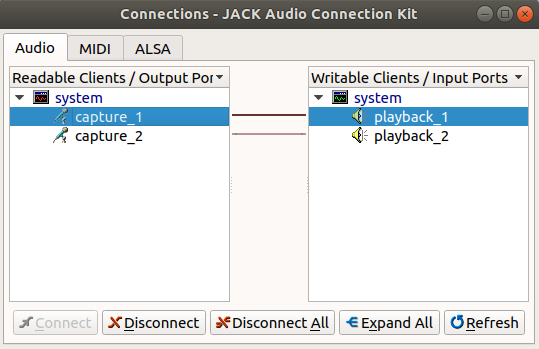
\includegraphics[scale=0.4]{jack_connection.png}
\caption{Jack GUI: Setup}
\label{fig: jack_connection}
\end{figure}


You can now use the JACK server as audio backend. For this, start openMHA in the same directory as before:

\item Open your \textbf{terminal} (see \ref{starting_openmha})
    \item \textbf{Navigate inside the examples folder into the subdirectory of the first example $\rightarrow$ \textbf{00-gain}} \\ (e.g. \textit{/home/YourUserName/Documents/examples/00-gain} )\\ \\
    $\rightarrow$ you can use \textbf{cd ..} to navigate one folder level higher \\
    $\rightarrow$ and \textbf{cd foldername} to navigate one folder level down
    \item Type {{\ttfamily mha \texttt{-{}-}interactive}} and press \textbf{Enter}
 
    %\item $\rightarrow$ {\ttfamily ?read:\textbackslash Users\textbackslash YourUserName\textbackslash Documents\textbackslash examples\textbackslash 00-gain\textbackslash \\ gain\_live.cfg}
\item $\rightarrow$ {\ttfamily ?read:gain\_live.cfg}
    \item $\rightarrow$ {\ttfamily cmd=start}

OpenMHA is now applying a gain to your own voice input. In order to close openMHA type:
\item  $\rightarrow$ {\ttfamily cmd=quit}

\end{enumerate}

\textcolor{orange}{\textbf{You have now managed to start some simple configurations for a static audio file as well as a live input using Jack. In the next session Matlab will be used as GUI for openMHA.}}


\newpage

\begin{comment}
\section{The remote connection - openMHA}
\label{sec_remote}

OpenMHA is now running and can be reached by default using port 33337. In order to communicate with OpenMHA you can use the network client \textbf{\textit{Netcat.}} Use a \textbf{second terminal windows} and type: \\
$\rightarrow$ \textbf{{\ttfamily nc localhost 33337}} 

For more details look into "openMHA\_application\_manual.pdf" (p. 4-7)\footnote{\label{foot:1}\url{https://github.com/HoerTech-gGmbH/openMHA/blob/master/openMHA_application_manual.pdf}}. \\

    Open a second terminal  \\
    Connect to openMHA using Netcat by typing: {\ttfamily nc localhost 33337}

\end{comment}



\section{Control Frequency Shifter using Octave/Matlab GUI}
\label{sec:freqshifter}

%During the openMHA installation process several Matlab functions were copied to the corresponding installation directory. In  the standard case you can find these Matlab function in \textbf{Program Files\textbackslash openMHA\textbackslash mfiles}.
%For this section you will make use of several openMHA Matlab function which you can find in \textit{/usr/lib/openmha/mfiles}. \textbf{Copy} these files to a non-protected directory, e.g. \textit{/home/YourUserName/Documents/}.



\begin{enumerate}
%\item Copy the \textbf{mfiles} folder into a non protected directory, e.g.
%\textbf{\textbackslash Users\textbackslash YourUserName\textbackslash
%Documents}
\item \textbf{End} all running \textbf{mha processes} 
\item \textbf{Open Matlab} 
\item Set LD\_LIBRARY\_PATH to empty by typing {\ttfamily setenv('LD\_LIBRARY\_PATH','')} into the \textbf{Command Window}
\item Use the Matlab \textbf{"Current Folder"} Section to navigate to:

\begin{itemize}
\item \textcolor{orange}{\textbf{Linux}}: \textit{/usr/share/openmha/examples/05-frequency-shifting} 
\item \textcolor{orange}{\textbf{Windows}}: \textit{C:\textbackslash Program Files\textbackslash openMHA\textbackslash examples\textbackslash 05-frequency-shifting}
\item \textcolor{orange}{\textbf{MacOS}}: \textit{/usr/local/share/openmha/examples/05-frequency-shifting} 
\end{itemize}

\item In order to use the Matlab functions of openMHA type the following using the \textbf{Command Window:} 

\begin{itemize}
\item \textcolor{orange}{\textbf{Linux}}: {\ttfamily addpath('/usr/lib/openmha/mfiles')}
\item \textcolor{orange}{\textbf{Windows}}: {\ttfamily addpath('C:\textbackslash Program Files\textbackslash openMHA\textbackslash mfiles')}
\item \textcolor{orange}{\textbf{MacOS}}: {\ttfamily addpath('/usr/local/lib/openmha/mfiles/')}
\end{itemize}


\item Use the Command Windows to enable communication with openMHA through java by typing: 

\begin{itemize}
\item \textcolor{orange}{\textbf{Linux}}: \\{\ttfamily javaaddpath('/usr/lib/openmha/mfiles/mhactl\_java.jar')} 
\item \textcolor{orange}{\textbf{Windows}}: \\ {\ttfamily addpath('C:\textbackslash Program Files\textbackslash openMHA\textbackslash mfiles\textbackslash mhactl\_java.jar')}
\item \textcolor{orange}{\textbf{MacOS}}: \\ {\ttfamily addpath('/usr/local/lib/openmha/mfiles/mhactl\_java.jar')}
\end{itemize}

%\item \textbf{Start openMHA} in the directory where \textbf{fshift\_live.cfg} is stored
%\item In order to create a handle, type in the following into the Matlab \textbf{Command Window}: \\ {\ttfamily h = struct( 'port', 33337, 'host', 'localhost' );}
%\item You can now use this handle to connect to openMHA by typing \\ {\ttfamily mha = mha\_get( h, '' );} into the  Matlab \textbf{Command Window}
\item In order to start openMHA type {\ttfamily openmha = mha\_start;} 
\item In order to read in the configuration file type: \\ {\ttfamily mha\_query(openmha,'','read:fbc.cfg');}
\item \textbf{Start JACK Server} using \textbf{JACK Control}\\ (Setting: Sample Rate = 44100, Frames/Period = 64)
\item Start the mha process by typing {\ttfamily mha\_set(openmha, 'cmd', 'start' );}
\item \textbf{JACK Control}: Connect the input clients correctly
\item Start GUI by typing {\ttfamily mhagui\_generic(openmha)} into the \textbf{Command Window}
\begin{enumerate}
\item \textbf{mha ->open sub-parser}
\item \textbf{mhachain ->open sub-parser}
\item \textbf{fshift\_hilbert ->open sub-parser}
\item \textbf{df -> open vector<float>control}
\end{enumerate}
\item Play around with the settings of the GUI and have fun :)
\end{enumerate}

\newpage

\section{Control Dynamic Compression using Octave/Matlab GUI}

%As in section \ref{sec:freqshifter}: During the openMHA installation process several Matlab functions were copied to the corresponding installation directory. In  the standard case you can find these Matlab function in \textbf{Program Files\textbackslash openMHA\textbackslash mfiles}.

\begin{enumerate}
\item \textbf{End} all running \textbf{mha processes} (You can type \textbf{killall mha} in the terminal to any running mha processes)
\item \textbf{Open Matlab}
\item Set LD\_LIBRARY\_PATH to empty by typing {\ttfamily setenv('LD\_LIBRARY\_PATH','')} into the \textbf{Command Window}
\item Use the Matlab \textbf{"Current Folder"} Section to navigate to:

\begin{itemize}
\item \textcolor{orange}{\textbf{Linux}}: \textit{/usr/share/openmha/examples/01-dynamic-compression} 
\item \textcolor{orange}{\textbf{Windows}}: \textit{C:\textbackslash Program Files\textbackslash openMHA\textbackslash examples\textbackslash 01-dynamic-compression}
\item \textcolor{orange}{\textbf{MacOS}}: \textit{/usr/local/share/openmha/examples/01-dynamic-compression} 
\end{itemize}

\item In order to use the Matlab functions of openMHA type the following using the \textbf{Command Window:} 

\begin{itemize}
\item \textcolor{orange}{\textbf{Linux}}: {\ttfamily addpath('/usr/lib/openmha/mfiles')}
\item \textcolor{orange}{\textbf{Windows}}: {\ttfamily addpath('C:\textbackslash Program Files\textbackslash openMHA\textbackslash mfiles')}
\item \textcolor{orange}{\textbf{MacOS}}: {\ttfamily addpath('/usr/local/lib/openmha/mfiles/')}
\end{itemize}


\item Use the Command Windows to enable communication with openMHA through java by typing: 

\begin{itemize}
\item \textcolor{orange}{\textbf{Linux}}: \\{\ttfamily javaaddpath('/usr/lib/openmha/mfiles/mhactl\_java.jar')} 
\item \textcolor{orange}{\textbf{Windows}}: \\ {\ttfamily addpath('C:\textbackslash Program Files\textbackslash openMHA\textbackslash mfiles\textbackslash mhactl\_java.jar')}
\item \textcolor{orange}{\textbf{MacOS}}: \\ {\ttfamily addpath('/usr/local/lib/openmha/mfiles/mhactl\_java.jar')}
\end{itemize}

\item In order to start openMHA type {\ttfamily openmha = mha\_start;} 
\item Read in configuration into mha by \\ {\ttfamily mha\_query(openmha,'','read:dynamiccompression\_live.cfg')}
\item \textbf{Start JACK Server} using \textbf{JACK Control}\\ (Setting: Sample Rate = 44100, Frames/Period = 64)
\item In order to start the mha process type {\ttfamily mha\_set(openMHA,'cmd','start')}
\item In order to read out the current gaintable and relevant paramters type the following: \\
{\ttfamily gaintable = mha\_get(openmha,'mha.overlapadd.mhachain.dc.gtdata');}\\
{\ttfamily gtmin = mha\_get(openmha,'mha.overlapadd.mhachain.dc.gtmin');}\\
{\ttfamily gtstep = mha\_get(openmha,'mha.overlapadd.mhachain.dc.gtstep');}
\item Plot the I/O characteristics \\
{\ttfamily level\_in = ((1:size(gaintable,2))-1) * gtstep + gtmin;}\\
{\ttfamily level\_out = level\_in + gaintable;}
\item In order to plot in-and output level type {\ttfamily figure, plot(level\_in,level\_out)}
\item You can design your own gaintable in Matlab by using 
  {\ttfamily gaintable\_new = [...]}
  \begin{itemize}
  \item e.g. Squash all input levels to the same output level, infinite compression:
    \\ \texttt{gaintable\_new = [65;65;65;65] - level\_in;}
  \item e.g. noise gate, compressive region, output limit: \\
    \texttt{gaintable\_new = repmat(4,1,[0,25,5,-35]);}
  \item e.g. compress high frequency band only: ...
  \end{itemize}
\item In order to apply the new gaintable type \\
{\ttfamily mha\_set(openmha,'mha.overlapadd.mhachain.dc.gtdata',gaintable\_new);}
\item You can stop openMHA using {\ttfamily mha\_set(openmha,'cmd','quit')}
\item More complex gaintable example would be \\
{\ttfamily openMHA = mha\_start([],\{\},\{'?read:dynamiccompression\_live.cfg'\})}\\
{\ttfamily mha\_set(openMHA,'cmd','start')}
\item Start fitting GUI by typing {\ttfamily mhacontrol(openmha)}



\end{enumerate}

\end{document}

%%% Local Variables: 
%%% mode: latex
%%% TeX-master: "openMHA_application_manual"
%%% indent-tabs-mode: nil
%%% coding: utf-8-unix
%%% End:
